% Drawing 74/03-11 -- folder 74, batch 03, archive page 60 (PDF page 61).
% Transcription: deux traits issus d'un même point vers deux points de la colonne voisine.
% Kind: two strokes from one point. Method 2 (schematic redraw from the facsimile). Status: ok.
% Notes: Under « 3) »: two strokes from the same point to two points of the neighbouring column (same crop as 03-10).
% Coordinates: 1 unit = 1 mm = 1/100 of the crop width (bbox in page fractions: [0.2, 0.36, 0.85, 0.6]).
% Redrawn by Claude (claude-opus-5-5), issue #73, 2026-11-07; not checked by a human; not compiled (no TeX in the session).
% Rights: reproduces part of the work -- behind RENDER_TRANSCRIPTS, never published by itself.
\documentclass[tikz,border=3pt]{standalone}
\usepackage{amsmath,amssymb}
\usetikzlibrary{patterns,arrows.meta}
\tikzset{pencil/.style={black!45}, struck/.style={black!35}, mark/.style={circle,draw,inner sep=1.3pt}, pt/.style={circle,fill,inner sep=0.9pt}, opt/.style={circle,draw,fill=white,inner sep=1.1pt}}
\begin{document}
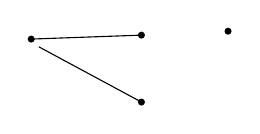
\begin{tikzpicture}[x=1mm,y=1mm,line cap=round,line join=round,font=\scriptsize]
\draw (20,-35) -- (34,-34.5);
\draw (21,-36) -- (34,-43);
\node[pt] at (20,-35) {};
\node[pt] at (34,-34.5) {};
\node[pt] at (34,-43) {};
\node[pt] at (45,-34) {};
\end{tikzpicture}
\end{document}
